\section{Volumetric displays}

Volumetric displays \cite{1492264} provide a three-dimensional viewing experience by emitting light from each voxel, or volume element, in a 3D space. This approach enables the accurate representation of virtual 3D objects while providing accurate focal depth, motion parallax, and vergence. Vergence refers to the rotation of a viewer's eye to fixate on the same point they are focusing on. Moreover, volumetric displays allow multiple users to view the same display from different angles, providing unique perspectives of the same object simultaneously.

\subsection{Advantages of Volumetric Displays Over 2D Displays and VR}

Volumetric displays offer distinct advantages over traditional 2D displays and virtual reality (VR). Unlike 2D displays, which only present flat images, volumetric displays create a true 3D experience by emitting light from each point in a 3D space. This allows viewers to perceive depth and see objects from different angles without the need for special glasses or head-tracking. \\

Compared to VR, volumetric displays do not require headsets, making them more accessible for multiple users simultaneously. This avoids the motion sickness and discomfort often associated with extended VR use \cite{doi:10.1080/10447318.2020.1778351}, providing a more natural and comfortable viewing experience. Volumetric displays can only present objects in the exact physical space they occupy, ensuring an accurate and grounded representation; however, unlike VR, they are unable to create a fully immersive experience.

\subsection{Swept Volume Displays}

\begin{invisBox}
  
	\pictureBox[label={fig:voxon}]{Voxon Photonics' VXR4612, a projector-based persistence of vision volumetric display. \cite{voxon2}}{
	  \adjustbox{height=4.7cm, keepaspectratio}{
		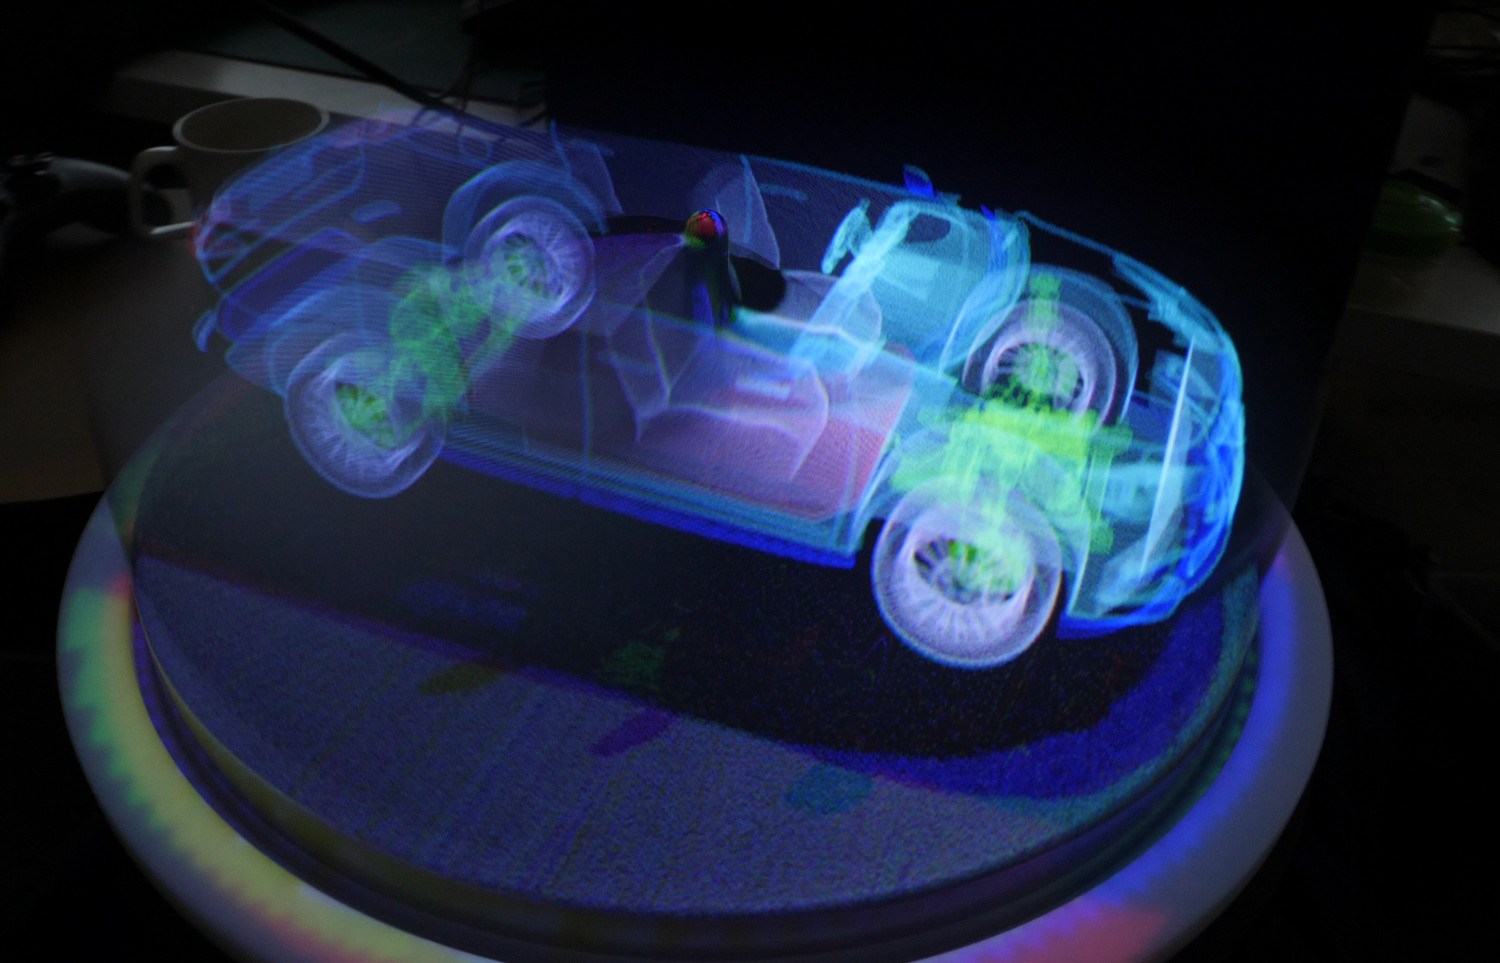
\includegraphics{./background/figures/3d/voxon.jpg}
	  }
	}
	\hfill
	\pictureBox[label={fig:brightbox}]{A Volumetric Display / Holographic Signage, an LED-based persistence of vision display produced by Brightvox Inc. \cite{brightvox_2023}}{
	\adjustbox{height=4.7cm, keepaspectratio}{
	  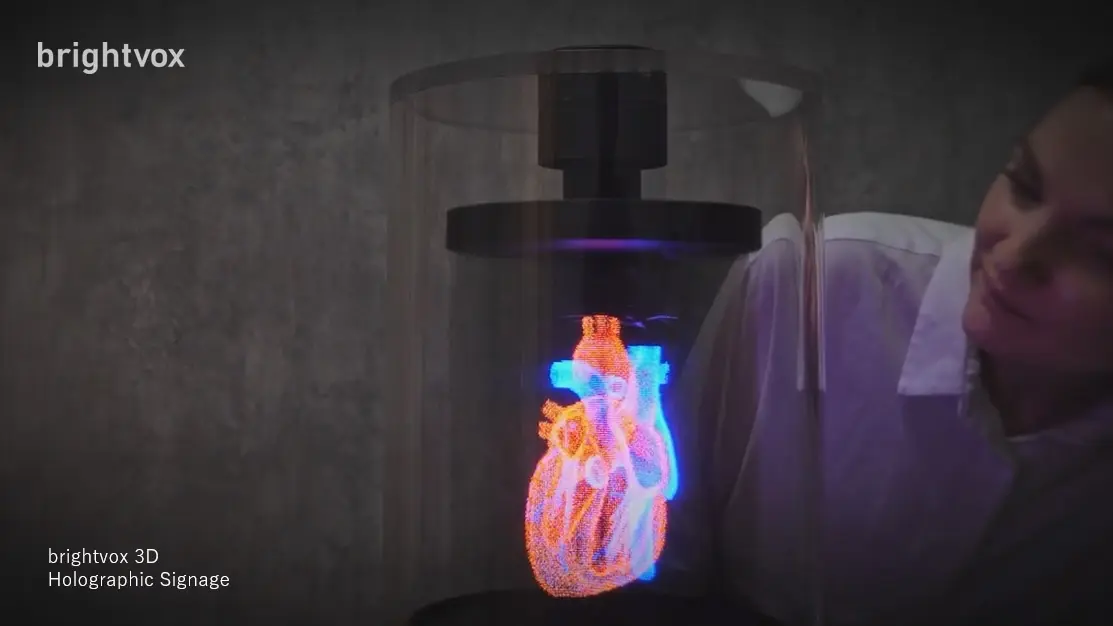
\includegraphics{./background/figures/3d/brightvox.png}
	  }
	}
\end{invisBox}  

Swept volume displays are one prominent category of volumetric displays. They employ a moving 2D display to create a 3D image through the persistence of vision effects. This is achieved by moving the 2D display through a 3D space at high speeds while emitting light from the display where it reaches the position of each corresponding voxel. Common techniques for achieving this include using a rotating mirror \cite{10.1117/12.480930}, an emitting screen, typically an LED-based \cite{Gately:11}, or a transparent projector screen \cite{keane_volumetric_2016}. There currently exist commercial products that implement this technique as can be seen in Fig~\ref{fig:voxon} and Fig~\ref{fig:brightbox}.


\subsection{Static Volume Displays}
Static volume displays are another category. They employ a static transparent medium that when interacted with creates a 3D image. The result is that light is emitted from the display at each point in a 3D space. Techniques for achieving this range from using a 3D array of LEDs \cite{10.1145/2341931.2341937}, lasers and phosphorus gas \cite{https://doi.org/10.1002/anie.202003160}, or a transparent laser-induced damaged medium that can be projected into \cite{10.1145/1179849.1179982}. There has been research into photon-activated dye \cite{Patel2017} and even quantum dot-based displays \cite{Hirayama2015}. An example of one such display can be seen in Fig~\ref{fig:passive-optical}.

\subsection{Trapped Particle Displays}
Acoustic Trapping Displays displays are a relatively new category of volumetric displays. They employ a 3D array of particles that are suspended in air using acoustic levitation. \cite{10.1063/1.5113467} \cite{Hirayama2019} This is achieved by using an array of ultrasonic transducers to create a standing wave that can trap particles in the nodes of the wave. By moving the nodes of the wave through a 3D space and illuminating the particles with light, a 3D image can be created. \\

This technique is still in its infancy and can struggle to provide a convincing persistence of vision effect. Another direction some researchers have taken is to use a photophoretic trap to trap particles in air \cite{Smalley2018}. The advantage of this sort of display is that space that is not being used to display an object is empty and can be passed through. This is in contrast to swept volume displays/most static volume displays where the space not being used to display an object is filled with the display's hardware. An example of one such display can be seen in Fig~\ref{fig:acoustic}.

\begin{invisBox}
	\pictureBox[label={fig:passive-optical}]{Columbia University's optical scattering volumetric display \cite{10.1145/1179849.1179982}}{
	  \adjustbox{height=5.7cm, keepaspectratio}{
		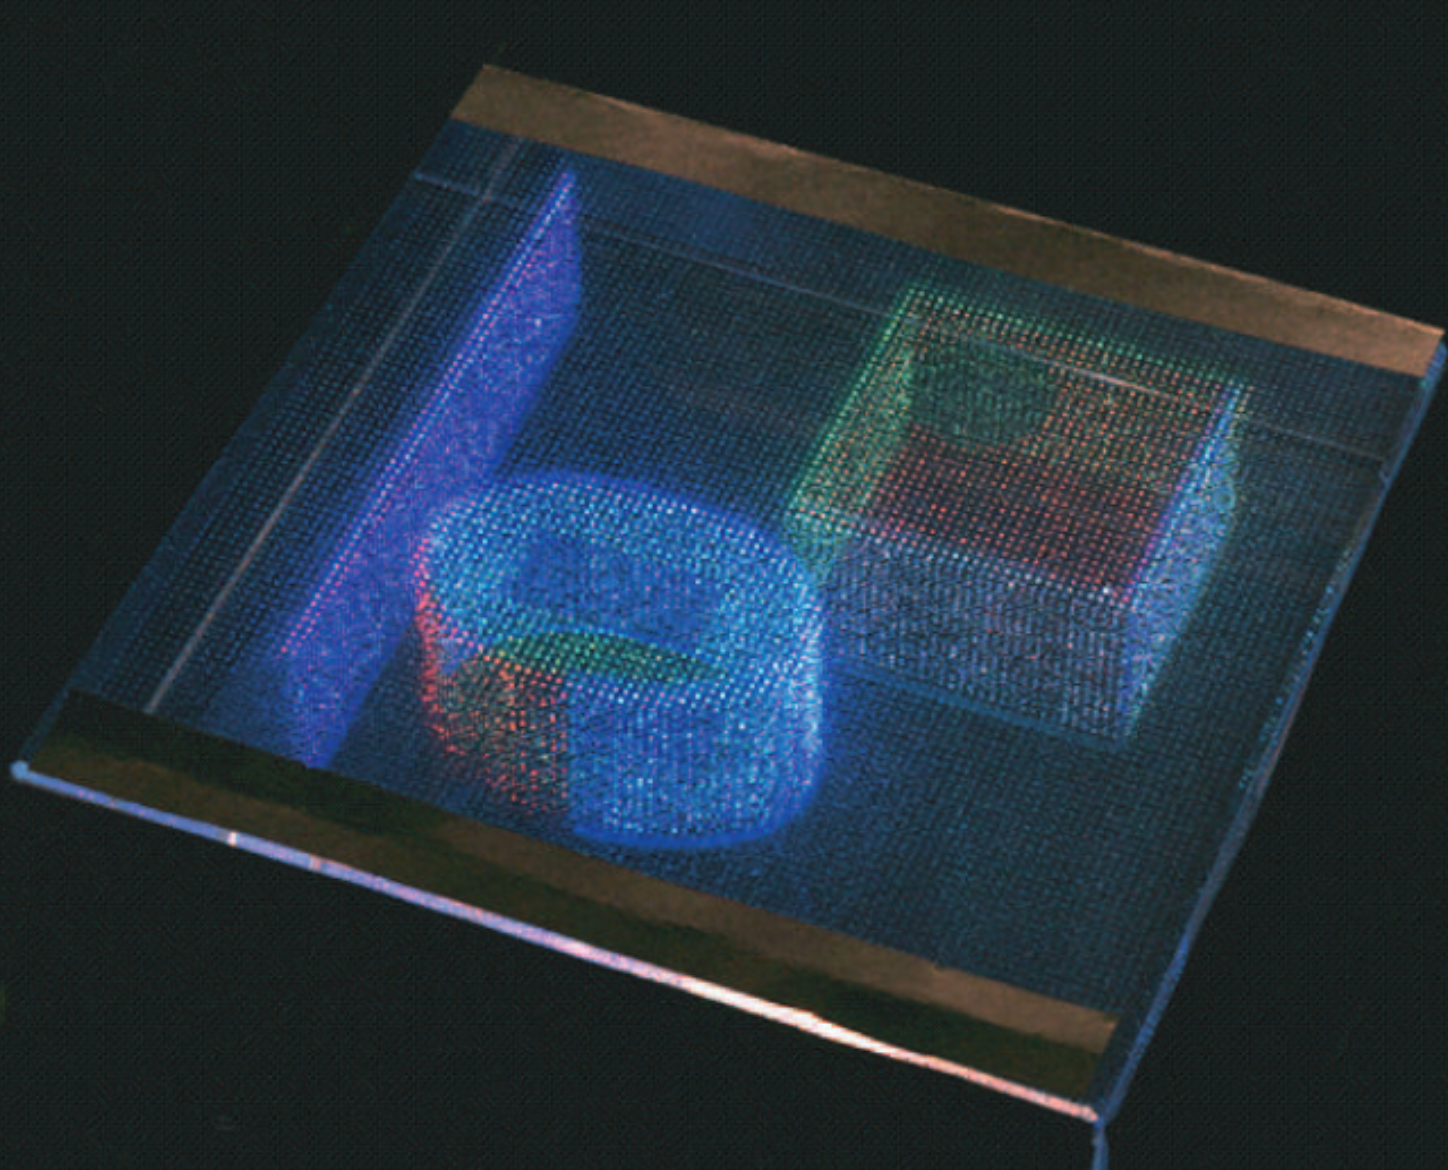
\includegraphics{./introduction/figures/passive optical scatterers.png}
	  }
	}
	\hfill
	\pictureBox[label={fig:acoustic}]{Bristol University's acoustic trapping volumetric display \cite{10.1063/1.5113467}}{
	\adjustbox{height=5.7cm, keepaspectratio}{
	  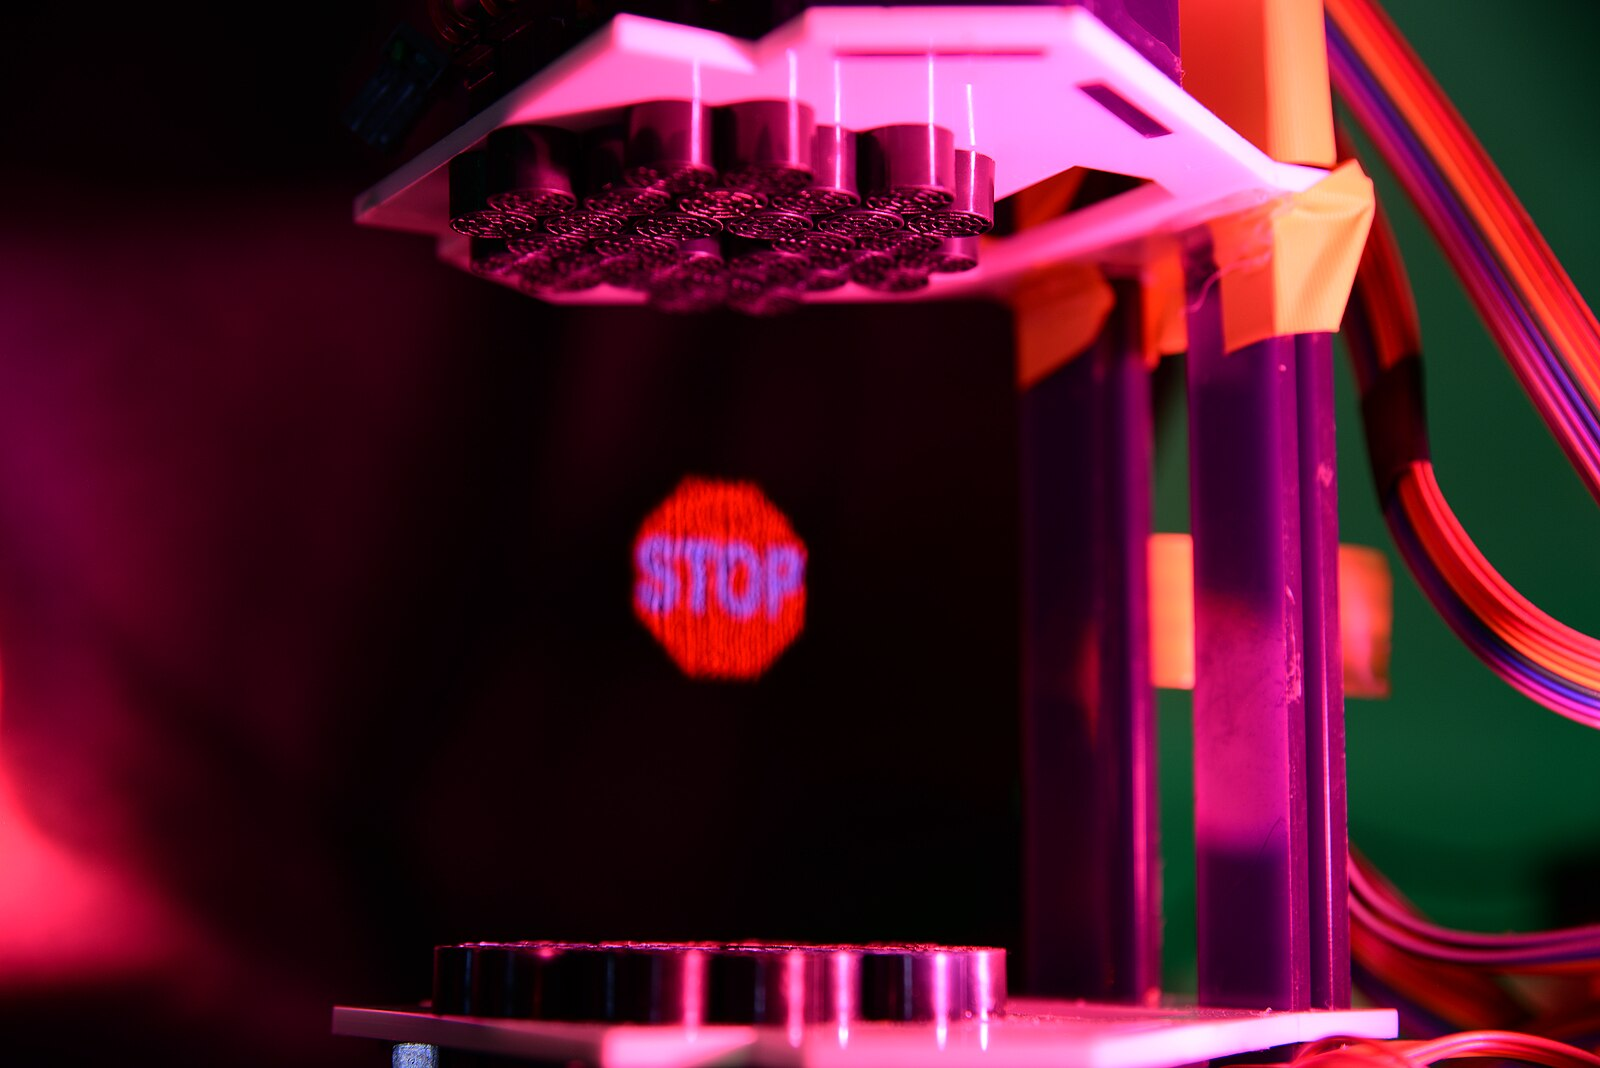
\includegraphics{./introduction/figures/acoustophoretic display.jpg}
	  }
	}
	\end{invisBox}
\subsection{Issues}

Volumetric displays often require custom/cutting-edge hardware (e.g. extremely high refresh rate projectors,  transparent micro LEDs, complex laser systems) which makes them expensive, difficult to manufacture and calibrate and not widely available. For example, the Voxon VX1, one of the few if only commercially available volumetric displays costs, \$11,700 USD \cite{noauthor_products_nodate} per unit. \\

Volumetric displays are also held back by their inherent high bandwidth requirements: To render objects in real-time at equivalent resolutions to current 2D displays while taking a raw voxel stream (as opposed to calculating voxels on hardware from primitive shapes) has an extremely high bandwidth requirement. If we want to render at \texttt{60fps} on a $4096 \times 2160 \times 1080$ voxel display with \texttt{24 bit} colour, it would require a bandwidth of $1.37 \times 10^3$ bits per second/13.7 terabits per second which is orders of magnitude higher than what a normal display requires. To achieve that currently would require about 170 state-of-the-art Ultra High Bit Rate (UHBR) (80 gigabit) DisplayPort cables simultaneously. It was predicted in 2021 \cite{LAM2021050011} that due to these limitations and based on the historic trends of bandwidth in commercially available displays, volumetric displays will only become feasible in 2060 at the earliest. There are ways to reduce this bandwidth requirement through compression and other techniques \cite{4487481} but this still provides a major issue. 

\section{Volumetric Display Simulations}
Due to the challenges associated with physical volumetric displays, significant research has been conducted into simulating these displays. These simulated displays are often referred to as fish tank virtual reality (FTVR) displays \cite{10.1145/169059.169066}. Although FTVRs were not originally designed to simulate volumetric displays, they have recently been adapted for research in this domain \cite{10.1145/3281505.3281540}, \cite{Zabarauskas2012}. An FTVR setup typically consists of one or more 2D displays (often curved into a concave shape) positioned in front of the user. The viewer's eye movements are tracked in 3D space, and the image on the displays is adjusted accordingly to create the illusion of a 3D image. \\

Figure~\ref{fig:crystal} and Figure~\ref{fig:mpCubee} illustrate two different approaches to FTVRs. The first, the CRSYSTAL Display \cite{noauthor_crystal_nodate}, employs a semi-transparent sphere illuminated from the inside by multiple projectors. The second, mpCubee \cite{7892378}, utilises multiple sets of mobile phones to achieve a similar effect.

\begin{invisBox}
    \pictureBox[label={fig:crystal}]{University of British Columbia's CRSYSTAL Display \cite{noauthor_crystal_nodate}}{
      \adjustbox{height=7.5cm, keepaspectratio}{
        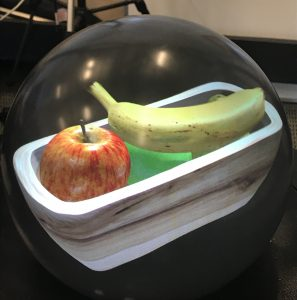
\includegraphics{./background/figures/3d/banana.jpg}
      }
    }
    \hfill
    \pictureBox[label={fig:mpCubee}]{Coburg University's and University of Passau's mpCubee \cite{7892378}}{
    \adjustbox{height=7.5cm, keepaspectratio}{
      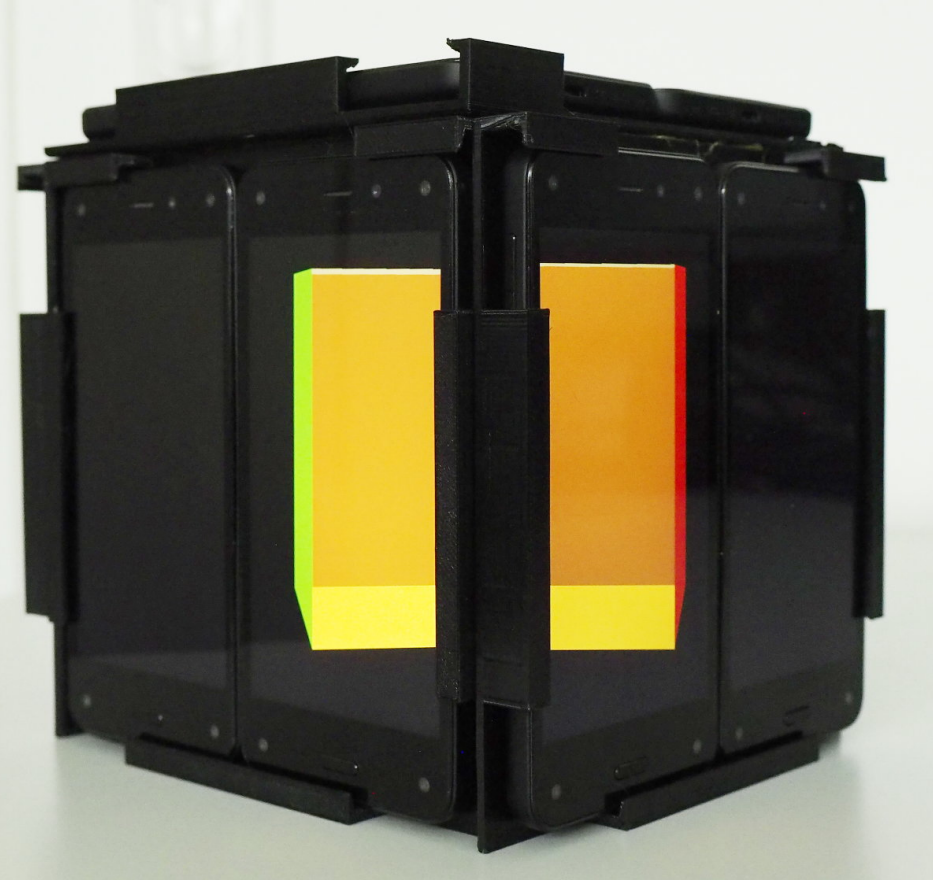
\includegraphics{./background/figures/3d/cubee.png}
      }
    }
\end{invisBox}

These solutions have several significant drawbacks. The user is constrained to a single focal depth and a single vergence. This limitation can be mitigated by using glasses that filter different images to each eye, providing a stereoscopic view \cite{5701756}. Additionally, these systems are generally limited to a single user at a time unless image filtering techniques are employed. Recreating these devices often requires a substantial collection of specialised tracking hardware and custom-built display components. \\

There have been several attempts to simulate volumetric displays using virtual reality (VR) headsets. VR headsets offer a relatively affordable and straightforward method for simulating volumetric displays and are capable of providing a stereoscopic view \cite{10.1145/3290605.3300763}. Historically, these devices have faced challenges with passthrough latency. However, recent advancements have significantly reduced this issue \cite{10.1145/3290605.3300763}, particularly with the introduction of devices like Apple's Vision Pro \cite{noauthor_apple_vision_nodate}. We believe this area holds considerable promise for future research. \\

